\documentclass[12pt,a4paper]{report}
\usepackage[utf8]{inputenc}
\usepackage[english]{babel}
\usepackage{amsmath}
\usepackage{amsfonts}
\usepackage{amssymb}
\usepackage{graphicx}
\usepackage{caption}
\usepackage{subcaption}
\usepackage{hyperref}
\graphicspath{ {image/} }
\usepackage[left=2cm,right=2cm,top=2cm,bottom=2cm]{geometry}
\bibliographystyle{ieeetran}

\author{HUYNH Le Duy}

\begin{document}

\tableofcontents

\listoffigures

\chapter{Theoretical Background}
\section{Digital Topology and Self-Duality}
\paragraph{}
A self-dual operator processes the image contents regardless its contrast \cite{Geraud.15.ismm}. In general, operators that are not self-dual do not treat bright objects over dark background and dark objects over bright background similarly which is often an undesirable feature. It is most important when no assumption about the contrast between object and background can be made. As any part of the images could be the subject, we want an operation which behavior the same way regardless the contrast between the subject and its background to obtain a unique representation.  
\begin{figure}

	\begin{subfigure}{0.3\textwidth}
	 	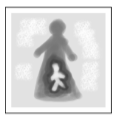
\includegraphics{im1.png} \caption{}\label{fig:gray} \end{subfigure}
	\begin{subfigure}{0.3\textwidth}
		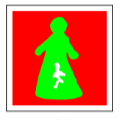
\includegraphics{im2.png} \caption{}\label{fig:mother} \end{subfigure}
	\begin{subfigure}{0.3\textwidth}
		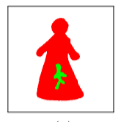
\includegraphics{im3.png} \caption{}\label{fig:baby} \end{subfigure}
	\centering
	\caption[Example of \textit{subjects}] {From the original gray level image \ref{fig:gray}, the subject can be either the mother \ref{fig:mother} (dark over bright) or the baby \ref{fig:baby} (bright over dark) }
	\label{fig:motheAndBaby}
\end{figure}

\paragraph{}
As we can seen in \ref{fig:motheAndBaby}, where green and red respectively represent the background and foreground. From the grayscale image \ref{fig:gray} If we focus in the mother, then the outer zone will be the background as in \ref{fig:mother}. Furthermore, we can chose the baby as the subject and therefore, the woman will become the background \ref{fig:baby}.	
\paragraph{}
For a image defined in the regular cubical grid, the digital topology must be describe by a "Jordan pair" of connectivity $(c_\alpha,c_\beta)$ \cite{Kong:1989:DTI:71397.71400}. One connectivity is used for the object and the other one for the background. This arbitrary choice affect the topology and self-dual operation must use different connectivity for the complementation to work in the same way.




\section{Well-composed Images}
\paragraph{}
As defined in \cite{Latecki95}, a 2D set S is weakly well-composed if any 8-component of S is a 4 component. S is well-composed if both S and its complement $\bar{C}$ are weakly well-composed. It can also be defined using the notion of "critical configurations" which are 
\includegraphics{confi1.jpg} and 
\includegraphics{confi2.jpg} : S is weakly well-composed if these configuration do not appear.
\paragraph{}
The notion of well-composednessed has also been extended to gray-level images. A gray-level image $\mu$ is well-composed if any set $[\mu \geq \lambda ]$ is well-composed. The extended version of "critical configuration" is that every block 
\begin{tabular}{|c|c|}
\hline 
a & d \\ 
\hline 
c & b \\ 
\hline 
\end{tabular} 
must verify interval(a,b) $\cap$ interval(c,d) $\neq \varnothing$ , where interval(a,b) = [min(a,b),max(a,b)].
\paragraph{}
An image is not a priori well-composed. There are 2 approach to get a well-composed image from the original image \cite{Geraud.15.ismm} by changing it pixel value (with possibility of alter the image's topology) or by a well-composed interpolation.



\section{Connected filter}
Motivated by families of filters by reconstruction, the notion of filter by reconstruction is introduced in \cite{Salembier95flatzones} \cite{Serra1993}. It work by simplifier the topographic map of images. The most important feature of this type of operator is preservation of contours \cite{Salembier2009}: they does not create new contours nor shift them.
\subsection{Morphological Tree-Based Image Representation}
One strategy to define connected operators replies on a hierarchical region-based representation of the input image, in another word, a tree. The filtering step is done by pruning that tree and the output image is compute by reconstructing the pruned tree.  Tree of shapes is a contrast-invariant image representation which is defined in \cite{Monasse.2000}.
\paragraph{} \textbf{A Couple of Dual Trees}: given an image $\mu $ in nD: $\mathbb{Z}^{n} \rightarrow \mathbb{Z} $, the lower cuts of $\mu$ are defined by 
	$[\mu < \lambda] =\lbrace x \in X \vert \mu (x) < \lambda \rbrace $. The set of all connected components of all these cuts is $ \mathcal{T}_< (\mu) =\lbrace \Gamma \in \mathcal{C}\mathcal{C}([\mu < \lambda]) \rbrace $ (with $\mathbb{C}\mathbb{C}$ denote the operator that takes a set and gives its set of connected component. As these sets verify $\forall \Gamma$ and $\Gamma ' \neq \lambda$, $\Gamma \subset \Gamma ' $ or $\Gamma \cap \Gamma '= \emptyset$, they can be arranged into a tree, called the \textit{min-tree} (because it if form using lower cuts, and the leaves will be minimum of image). We can also consider the upper cuts $[\mu \geq \lambda] =\lbrace x \in X \vert \mu (x) \geq \lambda \rbrace $, the element of $ \mathcal{T}_\geq (\mu) =\lbrace \Gamma \in \mathcal{C}\mathcal{C}([\mu \geq \lambda]) \rbrace $ will be arranged in to the \textit{max-tree}. The \textit{max-tree} and \textit{min-tree} are dual by complementation, the max-tree of $\mu$ is the min-tree of $ \mu$, therefore operations define on them are dual.
\paragraph{} \textbf{A Self-Dual Tree}:We use two set $ \mathcal{T}_< (\mu)$ and $ \mathcal{T}_\geq (\mu)$ with their holes filled to define two other sets $ \mathcal{S}_< (\mu)$ and $ \mathcal{S}_< (\mu)$. We denote \textit{Sat} as the cavity-fill-in operator, these new sets are defined as: $ \mathcal{S}_< (\mu) = \lbrace Sat(\Gamma);\Gamma \in \mathcal{T}_<(\mu)\rbrace$ and $ \mathcal{S}_\geq (\mu) = \lbrace Sat(\Gamma);\Gamma \in \mathcal{T}_\geq (\mu)\rbrace$. The tree of shape is defined as: $\mathfrak{S}(\mu) = \mathcal{S}_< (\mu) \bigcup \mathcal{S}_\geq (\mu) $. We have also $\Gamma \subset \Gamma ' $ or $\Gamma \cap \Gamma '= \emptyset$ with $\Gamma , \Gamma ' \in \mathcal{S}$. There is a quasi-linear algorithm to compute the tree of shape, which works also in the case of nD presented in \cite{geraud.13.ismm}. This tree is \textit{self-dual} because many self dual operation can be defined in this tree \textit{<reading article>}  .
	
\paragraph{To be continue... (consider add the attribute and definition of Sat)}

\chapter{Approach} \label{Approach}
\section{The simple morphological tree-based framework for image representation}
\paragraph{}
The morphological tree can be use to represent the image contents. Using the information carried by that tree, we can keep only interesting elements such as text. To compute a representation tree, mathematical morphology requires at first an order function of pixel values. In the case of color images, since there is not a natural order of color, the definition of is important and affect the performance. A classical workaround is to sort using their luminance by converting color image to gray-level image. 
\paragraph{}
A first possible approach is to compute the tree of shapes of the luminance, since a visible text must have a “dark over bright” contrast or the opposite one. Each note of this tree is a zone which have similar value.
\paragraph{}
A second possible approach base on the Laplacian morphology on the gray-level image. The zero-crossing of the laplacian are closed-contours and mark the boundary of object. By using laplacian morphology, we can distinguish object from the background. The size of objects conserved is depend on the windows using. Remind that the Laplacian morphology is calculate by $ \Delta_\Box = \delta_\Box + \varepsilon_\Box -2id $ as defined in \cite{Vliet_anedge}. The structure of the tree of shapes of the Laplacian is:
\begin{itemize}
\item A zone negative or positive will form a note
\item A zero point included in another note will belongs to that note
\item A note included in another note is a descendant of the former note
\end{itemize}
\paragraph{}
The tree of shapes of the Laplacian representation of region having similar luminance and their inclusion relationship. This tree is a light tree-base representation and well-suitable for some application such as image simplification [<give an example>] or smart binarization. 

\chapter{Implementation}

This chapter will clarify the implementation of the approach present in \autoref{Approach}.

\section{Well-composed Interpolation}

about the well composed implementation by median, multiple by 2, the important of sign

\section{Objects labeling}

\subsection{Labeling by front propagation}
\paragraph{} From the well-composed interposed laplacian, we will label all connected regions by front propagation. A region includes all pixel that has same sign of laplacian and zeros that touch that region. By that definition, the zeros will always belong to the outer region and invariant to the contrast between 2 regions therefore this operation is self-dual. 
\paragraph{}As we only interest in the sign of the Laplacian, a region is always surrounded by only one other region. We construct at the same time the tree-of-shape as a table of parents instead of an image with the same size as original image as in \cite{geraud.13.ismm}. 

\subsection{Average gradient calculation}
\paragraph{} We aim to remove and merge notes which has low contrast with the upper note. These notes will have low gradient in the contour, by calculate average gradient of thess points, we can decide which note to remove.There are many approach to obtain the contour, for example we can use a dilation follow by a erosion using a element cross as structure element to obtain the contour. But the calculation of erosion and dilation costs, so we want a simple contour following method. 
\paragraph{} For every new region detected except the first one (root), we will first follow the outer contour of the object to calculate its average gradient. As we read the image from left to right, top to bottom, first point of new region is always the left top most point. We initialize the starting point is the one on its left and initial last-direction is 0 (direction are numbered as in \ref{directionToSearch}). We test 8 possible direction of next point to find the one which is in labeled region and has the new region on its right. The searching order is a semicircle clockwise from last-direction plus a semicircle counter clockwise from last-direction. We continue until reaching the starting point. 
\begin{figure}
\begin{tabular}{|c|c|c|}
\hline 
6 & 7 & 0 \\ 
\hline 
5 & * & 1 \\ 
\hline 
4 & 3 & 2 \\ 
\hline 
\end{tabular}  
\centering
\caption{Possible positions of next point}
\label{directionToSearch}
\end{figure}

\begin{thebibliography}{9}
\bibitem{Latecki95}
    {Longin Latecki and Ulrich Eckhardt and Azriel Rosenfeld},
    {Well-Composed Sets},
    {Computer Vision and Image Understanding},
    {1995},
    {61},
    {70--83}
    
\bibitem{Vliet_anedge}
	{Lucas J. Van Vliet and Ian T. Young and Guus L. Beckers},
    {AN EDGE DETECTION MODEL BASED ON NON-LINEAR LAPLACE FILTERING},
    Pattern Recognition and Artificial Intelligence,
    pp. 63-73,
    1988.  
\bibitem {Geraud.15.ismm}
  {Thierry G\'eraud and Edwin Carlinet and S\'ebastien Crozet},
  {Self-Duality and Digital Topology: Links Between the
		  Morphological Tree of Shapes and Well-Composed Gray-Level
		  Images},
  {Mathematical Morphology and Its Application to Signal and
		  Image Processing -- Proceedings of the 12th International
		  Symposium on Mathematical Morphology (ISMM)},
  {2015},
  {Lecture Notes in Computer Science Series},
  {9082},
  {Reykjavik, Iceland},
  {Springer},
  {J.A. Benediktsson and J. Chanussot and L. Najman and H.
		  Talbot},
  {573--584}.
\bibitem {Kong:1989:DTI:71397.71400}
	{Kong, T. Y. and Rosenfeld, A.},
	{Digital Topology: Introduction and Survey},
	{Comput. Vision Graph. Image Process.},
	{Dec. 1989},
	{48},
	{3},
	dec,
	{1989},
	{0734-189X},
	{357--393},
	{37},
	{Academic Press Professional, Inc.},
	{San Diego, CA, USA},    
\bibitem {geraud.13.ismm}
  	{Thierry G\'eraud and Edwin Carlinet and S\'ebastien Crozet
		  and Laurent Najman},
  	{A quasi-linear algorithm to compute the tree of shapes of
	{$n$-D} images.},
	{Mathematical Morphology and Its Application to Signal and
		  Image Processing -- Proceedings of the 11th International
		  Symposium on Mathematical Morphology (ISMM)},
	2013,
	{C.L. Luengo Hendriks and G. Borgefors and R. Strand},
	7883,
	{Lecture Notes in Computer Science Series},
	{Uppsala, Sweden},
	{Springer},
	{98--110}
  	
\bibitem {Monasse.2000}
	{Monasse, P. and Guichard, F.},
	{Image Processing, IEEE Transactions on},
	{Fast computation of a contrast-invariant image representation},
	{2000},
	{May},
	{9},
	{5},
	{860-872}
\bibitem{Caselles2001}
    {Caselles V. and Monasse P.},
    {Grain filters},
    {2001}	
\bibitem{Salembier95flatzones}
    {P. Salembier and J. Serra},
    {Flat Zones Filtering, Connected Operators, and Filters by Reconstruction},
    {IEEE Transactions on Image Processing},
    {1995},
    {4},
    {1153--1160}
\bibitem{Serra1993}
	{Serra, Jean C. and Salembier, Philippe},
	{Connected operators and pyramids},
	{Proc. SPIE},
	{2030},
	{65-76},
	{1993},
\bibitem{Salembier2009}
	{Salembier, P. and Wilkinson, M.H.F.},
	{Signal Processing Magazine, IEEE},
	{Connected operators},
	{2009},
	{November},
	{26},
	{6},
	{136-157}, 
\end{thebibliography}

\end{document}



